\documentclass{article}
\usepackage{bookmark}

\usepackage[utf8]{inputenc}
\usepackage[brazil]{babel}  % Define o idioma para português do Brasil
\usepackage{csquotes}       % Para lidar com aspas de maneira apropriada com babel
\usepackage{array}
\usepackage{amsmath}
\usepackage{xcolor}

\usepackage{amsmath}
\usepackage{xcolor}
\usepackage{listings}
% Configuração do estilo de código
\lstset{
  language=C,
  %basicstyle=\ttfamily\footnotesize,
  keywordstyle=\color{blue},
  commentstyle=\color{gray},
  stringstyle=\color{red},
  breaklines=true,
  frame=single,
  numbers=left,
  numberstyle=\tiny,
  numbersep=5pt,
  showstringspaces=false,
}


\usepackage{graphicx}       % Pacote para inserção de imagens

\usepackage{hyperref}       % Pacote para links clicáveis
\hypersetup{
    colorlinks=true,
    linkcolor=blue,
    urlcolor=blue,
}

\usepackage{enumitem}       % Pacote para personalização de listas

\usepackage{geometry}       % Pacote para ajustar margens

\geometry{                  % Definindo margens personalizadas (em centímetros)
  left=2.5cm,  % Margem esquerda
  right=2.5cm, % Margem direita
  top=2.5cm,   % Margem superior
  bottom=2.5cm % Margem inferior
}

\usepackage[backend=biber,style=ieee]{biblatex}     % Estilo ieee para bibliografia numerada
\addbibresource{ref.bib}                            % Arquivo .bib


\begin{document}

\begin{titlepage}
    \centering
    % Cabeçalho personalizado
    
\includegraphics[width=0.3\textwidth]{../../Topic1/Avaliativo/Imagens/Logo UFLA - Colorida chapada.png}

    \vspace*{2cm} % Espaçamento vertical antes do cabeçalho
    \Large
    Universidade Federal de Lavras\\
    PPGCC\\
    PCC508 – Sistemas Operacionais\\
    
    \vspace{2cm} % Espaço entre o cabeçalho e o título
    \huge % Define o tamanho da fonte do título
    \textbf{Tópico 5 Lista Avaliativa}
    
    \vfill % Adiciona um espaçamento flexível antes do rodapé (opcional)
    
    % Opcionalmente, você pode incluir seu nome e a data aqui
    \large
    Douglas Aquino T. Mendes\\
    \today % Insere a data atual
\end{titlepage}

\tableofcontents
\newpage

\section{Introdução}
Este documento tem como objetivo apresentar o desenvolvimento das atividades avaliativas para o tópico 5 da disciplina de Sistemas Operacionais, focando na implementação de códigos em linguagem C. Serão apresentadas as questões, a resolução, os códigos desenvolvidos, seguidos de uma explicação sobre sua lógica de funcionamento.

\section{Questões}

\subsection{Algoritmo de substituição de páginas ótimo}
\textbf{Pergunta:} 1) Poderíamos criar uma ferramenta para analisar cada um dos programas para prever quando cada página seria utilizada, de modo a  implementarmos o algoritmo de substituição de páginas ótimo? Explique.  \newline

\textbf{Resposta:}  \textcite[p. 144]{tanenbaum2021} dizem que a criação de uma ferramenta para analisar programas e prever o uso futuro de páginas, com o objetivo de implementar o algoritmo ótimo de substituição de páginas, é teoricamente possível, porém impraticável em sistemas reais. O algoritmo ótimo de substituição de página postula que, em uma falta de página, a página que levará mais tempo para ser referenciada novamente deve ser removida da memória. Este algoritmo levaria ao menor número possível de faltas de páginas, mas seu problema reside na impossibilidade de prever com precisão quando cada página será utilizada no futuro.Embora seja impossível prever o futuro uso das páginas em um sistema em tempo real, o autor sugere que é possível simular o algoritmo ótimo em um ambiente controlado.


\subsection{Not Recently Used}

\textbf{Pergunta:} 2) Explique o algoritmo de substituição de páginas Not Recently Used (não usada recentemente), apresentando um exemplo. \newline

\textbf{Resposta:}  O algoritmo de substituição de páginas Not Recently Used (NRU), é um algoritmo que visa remover páginas da memória com base em seu uso recente e estado de modificação. O NRU utiliza dois bits principais associados a cada página: o bit R (Referenciada) e o bit M (Modificada) \parencite[p. 145]{tanenbaum2021}.

Bit R (Referenciada): Este bit é configurado pelo hardware sempre que uma página é acessada, seja para leitura ou escrita. O sistema operacional limpa periodicamente o bit R para identificar páginas que não foram usadas recentemente.

Bit M (Modificada): Este bit é configurado pelo hardware quando ocorre uma escrita em uma página. Ele indica se a página foi modificada desde que foi carregada do disco. Com base nos valores dos bits R e M, o algoritmo NRU classifica as páginas em quatro classes:

\begin{itemize}
    
    \item Classe 0: Páginas não referenciadas e não modificadas.
    \item Classe 1: Páginas não referenciadas, mas modificadas.
    \item Classe 2: Páginas referenciadas, mas não modificadas.
    \item Classe 3: Páginas referenciadas e modificadas.
\end{itemize}

Quando ocorre uma falta de página, o algoritmo NRU seleciona aleatoriamente uma página para remoção da classe de menor ordem não vazia. A lógica por trás dessa escolha é que é preferível remover uma página modificada, mas não referenciada recentemente (Classe 1), do que uma página não modificada que está sendo utilizada ativamente (Classe 2).

\newpage
\paragraph {Exemplo do Algoritmo NRU\newline}

Imagine um sistema com 4 páginas na memória e a seguinte configuração de bits R e M, como ilustrado na tabela \ref{tab:ReM}:
\begin{table}[h!]
    \centering
    \begin{tabular}{|c|c|c|c|}
    \hline
    \textbf{Página} & \textbf{R} & \textbf{M} & \textbf{Classe} \\ \hline
    0 & 1 & 0 & 2 \\ \hline
    1 & 0 & 1 & 1 \\ \hline
    2 & 1 & 1 & 3 \\ \hline
    3 & 0 & 0 & 0 \\ \hline
    \end{tabular}
    \caption{Valores de exemplo para os bits R e M}
    \label{tab:ReM}
\end{table}

Se ocorrer uma falta de página neste momento, o algoritmo NRU escolheria aleatoriamente uma página da Classe 0. No caso, a única opção seria a página 3. Após a remoção da página 3, a nova página seria carregada em seu lugar, e seus bits R e M seriam inicializados de acordo com o estado da página. O algoritmo NRU é fácil de entender e implementar, e oferece um desempenho razoável, embora não seja ótimo.


\subsection{Least Recently Used}

\textbf{Pergunta:} 3) Considere o algoritmo de substituição de página “Least Recently Used” (LRU) implementado com um hardware que mantém uma matriz de n x n bits. No exemplo, n será de 4 bits. Agora imagine a seguinte ordem de referência: 3 3 2 1 2 3 0. Mostre a sequência de matrizes de acesso do LRU para a ordem dada. Qual página que seria escolhida para substituição, se fosse necessário retirar uma?  \newline

\textbf{Resposta: }O algoritmo de substituição de página Least Recently Used (LRU) pode ser implementado com uma matriz de bits n×nn×n, onde nn é o número de páginas na memória. Essa matriz é atualizada a cada acesso, de forma que a linha correspondente à página acessada tenha seus bits ajustados.

\begin{itemize}
    \item Cada elemento da matriz $M[i][j]$ representa se a página $i$ foi acessada mais recentemente que a página $j$. Se $M[i][j]=1$, significa que $i$ foi acessada mais recentemente que $j$.
    \item Quando uma página é acessada, a linha correspondente a essa página é definida com $1$ em todas as suas posições, e a coluna correspondente a essa página é definida com $0$.
\end{itemize}

Considerando $n=4$ (páginas 0, 1, 2 e 3), a matriz de acesso $M$ é uma matriz $4×4$ inicialmente zerada. Dada a ordem de referência $3, 3, 2, 1, 2, 3, 0$, as matrizes são atualizadas conforme descrito a seguir:


\[M_{inicial} =
\begin{bmatrix}
  0_{00} & 0_{01} & 0_{02} & 0_{03}\\
  0_{10} & 0_{11} & 0_{12}    & 0_{13}\\
  0_{20} & 0_{21} & 0_{22}    & 0_{23}\\
  0_{30} & 0_{31} & 0_{32}    & 0_{33}
\end{bmatrix}
\]

\[PaginaReferenciada: 3 =
\begin{bmatrix}
  0_{00} & 0_{01} & 0_{02} & \textcolor{blue}{0_{03}}\\
  0_{10} & 0_{11} & 0_{12}    & \textcolor{blue}{0_{13}}\\
  0_{20} & 0_{21} & 0_{22}    & \textcolor{blue}{0_{23}}\\
  \textcolor{red}{1_{30}} & \textcolor{red}{1_{31}} & \textcolor{red}{1_{32}}    & \textcolor{blue}{0_{33}}
\end{bmatrix}
\]

\[
PaginaReferenciada: 2 =
\begin{bmatrix}
  0_{00} & 0_{01} & \textcolor{blue}{0_{02}} & 0_{03} \\
  0_{10} & 0_{11} & \textcolor{blue}{0_{12}} & 0_{13} \\
  \textcolor{red}{1_{20}} & \textcolor{red}{1_{21}} & \textcolor{blue}{0_{22}} & \textcolor{red}{1_{23}} \\
  1_{30} & 1_{31} & \textcolor{blue}{0_{32}} & 0_{33}
\end{bmatrix}
\]

\[
PaginaReferenciada: 1 =
\begin{bmatrix}
  0_{00} & \textcolor{blue}{0_{01}} & 0_{02} & 0_{03} \\
  \textcolor{red}{1_{10}} & \textcolor{blue}{0_{11}} & \textcolor{red}{1_{12}} & \textcolor{red}{1_{13}} \\
  1_{20} & \textcolor{blue}{0_{21}} & 0_{22} & 1_{23} \\
  1_{30} & \textcolor{blue}{0_{31}} & 0_{32} & 0_{33}
\end{bmatrix}
\]

\[
PaginaReferenciada: 2 =
\begin{bmatrix}
  0_{00} & 0_{01} & \textcolor{blue}0_{02} & 0_{03} \\
  {1_{10}} & {0_{11}} & \textcolor{blue}{0_{12}} & {1_{13}} \\
  \textcolor{red}{1_{20}} & \textcolor{red}{1_{21}} & \textcolor{blue}{0_{22}} & \textcolor{red}{1_{23}} \\
  1_{30} & {0_{31}} & \textcolor{blue}{0_{32}} & 0_{33}
\end{bmatrix}
\]

\[
PaginaReferenciada: 3 =
\begin{bmatrix}
  0_{00} & 0_{01} & 0_{02} & \textcolor{blue}{0_{03}} \\
  {1_{10}} & {0_{11}} & {0_{12}} & \textcolor{blue}{0_{13}} \\
  {1_{20}} & {1_{21}} & {0_{22}} & \textcolor{blue}{0_{23}} \\
  \textcolor{red}{1_{30}} & \textcolor{red}{1_{31}} & \textcolor{red}{1_{32}} & \textcolor{blue}{0_{33}}
\end{bmatrix}
\]

\[
PaginaReferenciada: 0 =
\begin{bmatrix}
    \textcolor{blue}{0_{00}} & \textcolor{red}{1_{01}} & \textcolor{red}{1_{02}} & \textcolor{red}{1_{03}} \\
    \textcolor{blue}{0_{10}} & {0_{11}} & {0_{12}} & {0_{13}} \\
    \textcolor{blue}{0_{20}} & {1_{21}} & {0_{22}} & {0_{23}} \\
    \textcolor{blue}{0_{30}} & {1_{31}} & {1_{32}} & {0_{33}}
\end{bmatrix}
\]

Para identificar a página a ser substituída, verificamos a linha com o menor valor binário, pois ela não foi acessada a mais tempo em relação a todas as outras. Nesse caso, observando a matriz final, a página 1 seria escolhida para substituição, pois é a página com menor valor.

\subsection{Page Fault Frequency}

\textbf{Pergunta:} 4) O algoritmo PFF (Page Fault Frequency – Frequência de Falta de Página) é utilizado para controlar o tamanho do conjunto de páginas alocadas na memória RAM de um determinado processo, quando um algoritmo de alocação global é utilizado. Explique, com exemplos, como funciona este algoritmo.  \newline

\textbf{Resposta:}

\textbf{Pergunta:} 5) Explique como funciona a tradução de um endereço MULTICS para o endereço físico da máquina. O MULTICS trabalha com segmentação com paginação. Explique como funciona o descritor de segmento juntamente com as tabelas de páginas.  \newline

\textbf{Resposta:} 

\section{Desenvolver um programa}

\subsection{}
\textbf{Enunciado:} Nos dias atuais, sistemas com múltiplos cores dentro do processador estão em toda a parte. No Linux, podemos determinar a afinidade de uma determinada thread a um dado core com a função: sched-setaffinity. Faça um programa que gere 4 vertores de tamanho n com números aleatórios. Cada vetor deve ser ordenado por uma thread diferente. As threads devem ser divididas entre os cores existentes e cada thread deve sempre ser executada no mesmo core. Você deve verificar se a afinidade da thread foi escolhida corretamente com a função sched-getaffinity. Além disso, o comando top deve
ser utilizado para a verificação do core que executa cada thread. \newline

\subsection{Código}
\label{sub-sec-cod}
%\lstinputlisting[language=C]{Codes/atv1_sharedmem.c}
\subsection{Testes e Resultados}
Como resultado da execução do código exibido na subceção \ref{sub-sec-cod}, obtivemos a saída ilustrada na figura \ref{fig:exec}. É importante ressaltar que o programa pode apresentar um problema, pois não há verificação de produzir apenas quando há espaço, ou seja, o buffer pode acabar sendo subscrito pela função de produzir, antes da função de consumir. 

\begin{figure}[ht]
    \centering
    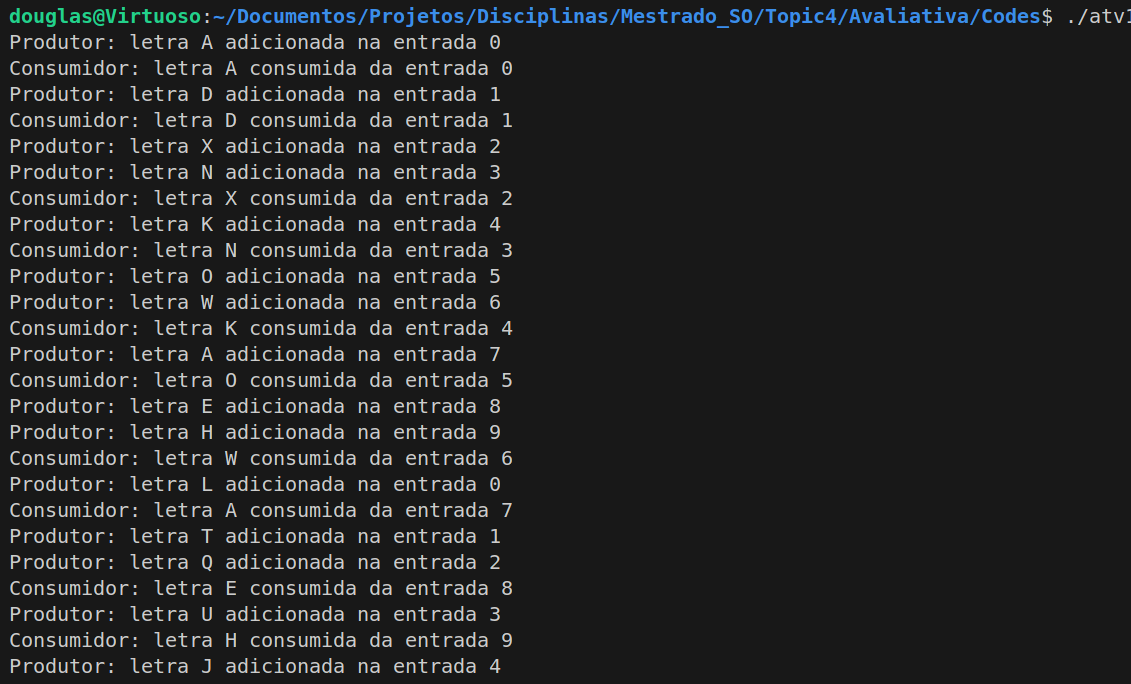
\includegraphics[width=1\textwidth]{./Images/image.png}
    \caption{Resultado da execução do programa}
    \label{fig:exec}
\end{figure}

\printbibliography % Imprime a lista de referências


\end{document}